% Options for packages loaded elsewhere
\PassOptionsToPackage{unicode}{hyperref}
\PassOptionsToPackage{hyphens}{url}
\documentclass[
  english,
  man,floatsintext]{apa6}
\usepackage{xcolor}
\usepackage{amsmath,amssymb}
\setcounter{secnumdepth}{-\maxdimen} % remove section numbering
\usepackage{iftex}
\ifPDFTeX
  \usepackage[T1]{fontenc}
  \usepackage[utf8]{inputenc}
  \usepackage{textcomp} % provide euro and other symbols
\else % if luatex or xetex
  \usepackage{unicode-math} % this also loads fontspec
  \defaultfontfeatures{Scale=MatchLowercase}
  \defaultfontfeatures[\rmfamily]{Ligatures=TeX,Scale=1}
\fi
\usepackage{lmodern}
\ifPDFTeX\else
  % xetex/luatex font selection
\fi
% Use upquote if available, for straight quotes in verbatim environments
\IfFileExists{upquote.sty}{\usepackage{upquote}}{}
\IfFileExists{microtype.sty}{% use microtype if available
  \usepackage[]{microtype}
  \UseMicrotypeSet[protrusion]{basicmath} % disable protrusion for tt fonts
}{}
\makeatletter
\@ifundefined{KOMAClassName}{% if non-KOMA class
  \IfFileExists{parskip.sty}{%
    \usepackage{parskip}
  }{% else
    \setlength{\parindent}{0pt}
    \setlength{\parskip}{6pt plus 2pt minus 1pt}}
}{% if KOMA class
  \KOMAoptions{parskip=half}}
\makeatother
% Make \paragraph and \subparagraph free-standing
\makeatletter
\ifx\paragraph\undefined\else
  \let\oldparagraph\paragraph
  \renewcommand{\paragraph}{
    \@ifstar
      \xxxParagraphStar
      \xxxParagraphNoStar
  }
  \newcommand{\xxxParagraphStar}[1]{\oldparagraph*{#1}\mbox{}}
  \newcommand{\xxxParagraphNoStar}[1]{\oldparagraph{#1}\mbox{}}
\fi
\ifx\subparagraph\undefined\else
  \let\oldsubparagraph\subparagraph
  \renewcommand{\subparagraph}{
    \@ifstar
      \xxxSubParagraphStar
      \xxxSubParagraphNoStar
  }
  \newcommand{\xxxSubParagraphStar}[1]{\oldsubparagraph*{#1}\mbox{}}
  \newcommand{\xxxSubParagraphNoStar}[1]{\oldsubparagraph{#1}\mbox{}}
\fi
\makeatother
\usepackage{graphicx}
\makeatletter
\newsavebox\pandoc@box
\newcommand*\pandocbounded[1]{% scales image to fit in text height/width
  \sbox\pandoc@box{#1}%
  \Gscale@div\@tempa{\textheight}{\dimexpr\ht\pandoc@box+\dp\pandoc@box\relax}%
  \Gscale@div\@tempb{\linewidth}{\wd\pandoc@box}%
  \ifdim\@tempb\p@<\@tempa\p@\let\@tempa\@tempb\fi% select the smaller of both
  \ifdim\@tempa\p@<\p@\scalebox{\@tempa}{\usebox\pandoc@box}%
  \else\usebox{\pandoc@box}%
  \fi%
}
% Set default figure placement to htbp
\def\fps@figure{htbp}
\makeatother
% definitions for citeproc citations
\NewDocumentCommand\citeproctext{}{}
\NewDocumentCommand\citeproc{mm}{%
  \begingroup\def\citeproctext{#2}\cite{#1}\endgroup}
\makeatletter
 % allow citations to break across lines
 \let\@cite@ofmt\@firstofone
 % avoid brackets around text for \cite:
 \def\@biblabel#1{}
 \def\@cite#1#2{{#1\if@tempswa , #2\fi}}
\makeatother
\newlength{\cslhangindent}
\setlength{\cslhangindent}{1.5em}
\newlength{\csllabelwidth}
\setlength{\csllabelwidth}{3em}
\newenvironment{CSLReferences}[2] % #1 hanging-indent, #2 entry-spacing
 {\begin{list}{}{%
  \setlength{\itemindent}{0pt}
  \setlength{\leftmargin}{0pt}
  \setlength{\parsep}{0pt}
  % turn on hanging indent if param 1 is 1
  \ifodd #1
   \setlength{\leftmargin}{\cslhangindent}
   \setlength{\itemindent}{-1\cslhangindent}
  \fi
  % set entry spacing
  \setlength{\itemsep}{#2\baselineskip}}}
 {\end{list}}
\usepackage{calc}
\newcommand{\CSLBlock}[1]{\hfill\break\parbox[t]{\linewidth}{\strut\ignorespaces#1\strut}}
\newcommand{\CSLLeftMargin}[1]{\parbox[t]{\csllabelwidth}{\strut#1\strut}}
\newcommand{\CSLRightInline}[1]{\parbox[t]{\linewidth - \csllabelwidth}{\strut#1\strut}}
\newcommand{\CSLIndent}[1]{\hspace{\cslhangindent}#1}
\ifLuaTeX
\usepackage[bidi=basic]{babel}
\else
\usepackage[bidi=default]{babel}
\fi
% get rid of language-specific shorthands (see #6817):
\let\LanguageShortHands\languageshorthands
\def\languageshorthands#1{}
\ifLuaTeX
  \usepackage[english]{selnolig} % disable illegal ligatures
\fi
\setlength{\emergencystretch}{3em} % prevent overfull lines
\providecommand{\tightlist}{%
  \setlength{\itemsep}{0pt}\setlength{\parskip}{0pt}}
% Manuscript styling
\usepackage{upgreek}
\captionsetup{font=singlespacing,justification=justified}

% Table formatting
\usepackage{longtable}
\usepackage{lscape}
% \usepackage[counterclockwise]{rotating}   % Landscape page setup for large tables
\usepackage{multirow}		% Table styling
\usepackage{tabularx}		% Control Column width
\usepackage[flushleft]{threeparttable}	% Allows for three part tables with a specified notes section
\usepackage{threeparttablex}            % Lets threeparttable work with longtable

% Create new environments so endfloat can handle them
% \newenvironment{ltable}
%   {\begin{landscape}\centering\begin{threeparttable}}
%   {\end{threeparttable}\end{landscape}}
\newenvironment{lltable}{\begin{landscape}\centering\begin{ThreePartTable}}{\end{ThreePartTable}\end{landscape}}

% Enables adjusting longtable caption width to table width
% Solution found at http://golatex.de/longtable-mit-caption-so-breit-wie-die-tabelle-t15767.html
\makeatletter
\newcommand\LastLTentrywidth{1em}
\newlength\longtablewidth
\setlength{\longtablewidth}{1in}
\newcommand{\getlongtablewidth}{\begingroup \ifcsname LT@\roman{LT@tables}\endcsname \global\longtablewidth=0pt \renewcommand{\LT@entry}[2]{\global\advance\longtablewidth by ##2\relax\gdef\LastLTentrywidth{##2}}\@nameuse{LT@\roman{LT@tables}} \fi \endgroup}

% \setlength{\parindent}{0.5in}
% \setlength{\parskip}{0pt plus 0pt minus 0pt}

% Overwrite redefinition of paragraph and subparagraph by the default LaTeX template
% See https://github.com/crsh/papaja/issues/292
\makeatletter
\renewcommand{\paragraph}{\@startsection{paragraph}{4}{\parindent}%
  {0\baselineskip \@plus 0.2ex \@minus 0.2ex}%
  {-1em}%
  {\normalfont\normalsize\bfseries\itshape\typesectitle}}

\renewcommand{\subparagraph}[1]{\@startsection{subparagraph}{5}{1em}%
  {0\baselineskip \@plus 0.2ex \@minus 0.2ex}%
  {-\z@\relax}%
  {\normalfont\normalsize\itshape\hspace{\parindent}{#1}\textit{\addperi}}{\relax}}
\makeatother

\makeatletter
\usepackage{etoolbox}
\patchcmd{\maketitle}
  {\section{\normalfont\normalsize\abstractname}}
  {\section*{\normalfont\normalsize\abstractname}}
  {}{\typeout{Failed to patch abstract.}}
\patchcmd{\maketitle}
  {\section{\protect\normalfont{\@title}}}
  {\section*{\protect\normalfont{\@title}}}
  {}{\typeout{Failed to patch title.}}
\makeatother

\usepackage{xpatch}
\makeatletter
\xapptocmd\appendix
  {\xapptocmd\section
    {\addcontentsline{toc}{section}{\appendixname\ifoneappendix\else~\theappendix\fi: #1}}
    {}{\InnerPatchFailed}%
  }
{}{\PatchFailed}
\makeatother
\keywords{College major choice, undergraduate students, locus of control, self-authorship\newline\indent Word count: 542}
\usepackage{csquotes}
\usepackage{bookmark}
\IfFileExists{xurl.sty}{\usepackage{xurl}}{} % add URL line breaks if available
\urlstyle{same}
\hypersetup{
  pdftitle={Changes in Locus of Control Orientation Across College Major Pathways},
  pdfauthor={Varsha Venkatesh1 \& Moin Syed1},
  pdflang={en-EN},
  pdfkeywords={College major choice, undergraduate students, locus of control, self-authorship},
  hidelinks,
  pdfcreator={LaTeX via pandoc}}

\title{Changes in Locus of Control Orientation Across College Major Pathways}
\author{Varsha Venkatesh\textsuperscript{1} \& Moin Syed\textsuperscript{1}}
\date{}


\shorttitle{Locus of Control and Major Pathways}

\authornote{

The authors made the following contributions. Varsha Venkatesh: Conceptualization, Writing - Original Draft Preparation, Writing - Review \& Editing; Moin Syed: Writing - Review \& Editing, Supervision.

Correspondence concerning this article should be addressed to Varsha Venkatesh, 75 E River Pkwy, Minneapolis, MN 55455. E-mail: \href{mailto:venka288@umn.edu}{\nolinkurl{venka288@umn.edu}}

}

\affiliation{\vspace{0.5cm}\textsuperscript{1} University of Minnesota}

\abstract{%
Choosing a college major is among the most important and difficult decisions that a student makes in their career. The present study seeks to better understand how feelings of control and agency can impact this choice. In particular, we do so by examining how locus of control changes among undergraduate students over the course of the first two years of college and how these patterns vary across different major pathways. The current student expands upon past research in three major ways. Firstly, previous studies of college student major choice more broadly compare undecided and decided students as opposed to narrower paths toward college major choice. Secondly, most previous studies of major choice examine group differences at one timepoint, rather than longitudinally. Finally, while locus of control has been extensively studied, there is a dearth of research on how locus of control changes over time, particularly among undergraduate students. Based on past studies of locus of control and decision-making as well as Baxter Magolda's theory of self-authorship, we hypothesized that across the five major pathways measured in this study (uncertain, discovery, redirect, solidification, and certain), we would observe varied longitudinal patterns of locus of control.
}



\begin{document}
\maketitle

Picking an undergraduate major, while always an important decision, has become increasingly complicated over the years. With an ever-changing job market and an expanding selection of academic programs, students have many external factors to consider when making this life-altering choice. Additionally, students must examine internal characteristics, such as skills, values, and interests. However, how students make this decision varies from person to person. While some students enter college confident in their choice and stick with it till graduation, many others come in undeclared or change their major at some point in their undergraduate career. These different ways of arriving at a college major, or major pathways, outline different patterns of decision-making that demand further investigation.

The present study seeks to better understand how feelings of control and agency impact academic decision-making. In particular, we do so by examining how locus of control changes among undergraduate students over the course of the first two years of college and how these patterns vary across different major pathways. The current student expands upon past research in three major ways. Firstly, previous studies of college student major choice more broadly compare undecided and decided students (Gordon, 1998; Rose \& Elton, 1971; Spight, Mooney, \& Orr, 2024) as opposed to narrower paths toward college major choice. Secondly, most previous studies of major choice examine group differences during a student's freshman year (Rose \& Elton, 1971; Spight et al., 2024), rather than longitudinally. Finally, while locus of control has been extensively studied, there is a dearth of research on how locus of control changes over time (Nowicki, Ellis, Iles-Caven, Gregory, \& Golding, 2018).

Based on past studies of locus of control and decision-making as well as self-authorship theory (Magolda, 2023), we hypothesize that across the five major pathways measured in this study (uncertain, discovery, redirect, solidification, and certain), we would observe varied longitudinal patterns of locus of control. As locus of control was measured continuously--- with lower scores indicating externality and higher scores indicating internality--- hypotheses were based on both orientation at Time 1 (T1) and change from T1 to Time 4 (T4). Specifically, we hypothesize that 1) students in the uncertain pathway will demonstrate stable external locus of control from T1 to T4, 2) students in the discovery pathway will demonstrate a shift from external locus of control to internal locus of control between T1 to T4, 3) students in the redirect pathway will show stable internal locus of control from T1 to T4, 4) students in the solidification pathway will demonstrate increased internality from T1 to T4, and 5) students in the certain pathway will show stable internal locus of control from T1 to T4.

\section{Method}\label{method}

\subsection{Participants and Procedure}\label{participants-and-procedure}

Participants were 96 undergraduate students enrolled at a large, public university in the United States. They ranged in age from 18 to 22 years old (\emph{M} = 18.91, \emph{SD} = 1.15). The majority of participants identified as Asian/Pacific Islander (34.38\%) and male (55.21\%). Additionally, the majority (96.88\%) of participants were born in the United States. A detailed summary of participant demographics is available in Table 1.

\begin{table}[tbp]

\begin{center}
\begin{threeparttable}

\caption{\label{tab:descriptive table}Sociodemographic Characteristics of Participants}

\begin{tabular}{lll}
\toprule
Characteristic & \multicolumn{1}{c}{n} & \multicolumn{1}{c}{\%}\\
\midrule
Gender &  & \\
\ \ \ \  Male & 53 & 55.21\\
\ \ \ \  Female & 40 & 41.67\\
\ \ \ \  Nonbinary & 3 & 3.12\\
Race &  & \\
\ \ \ \  Asian/Pacific Islander & 33 & 34.38\\
\ \ \ \  Black/African American & 24 & 25\\
\ \ \ \  Hispanic/Latine & 16 & 16.67\\
\ \ \ \  Multiracial & 12 & 12.5\\
\ \ \ \  Native American & 7 & 7.29\\
\ \ \ \  Other & 4 & 4.17\\
Birthplace &  & \\
\ \ \ \  Born in the US & 93 & 96.88\\
\ \ \ \  Not Born in the US & 3 & 3.12\\
\bottomrule
\addlinespace
\end{tabular}

\begin{tablenotes}[para]
\normalsize{\textit{Note.} N = 96. Participants were 18.91 years old on average (SD = 1.15)}
\end{tablenotes}

\end{threeparttable}
\end{center}

\end{table}

Participants were recruited through a multicultural orientation event, with the first wave of data collection occurring prior to their first semester of college and the final wave occurring during the second semester of their sophomore year. They completed the first wave of the study as part of student orientation. The following three waves of the study were sent via email, and participants received \$7 per completed follow-up survey. Those who participated in at least three waves of the survey were included in analyses.

\subsection{Materials}\label{materials}

\subsubsection{College Major Pathway}\label{college-major-pathway}

College major pathways were coded based on participant self-reported narratives about their path to choosing a college major. Students were assigned one of five pathways: Uncertain (uncertain of their major from T1 to T4), Discovery (undecided at T1, chose major by T4), Redirect (changed major between T1 and T4), Solidification (unsure about initial major at T1, certain about same major at T4), and Certain (certain about same major from T1 to T4).

\subsubsection{Locus of Control}\label{locus-of-control}

Locus of control was measured through the Internal Locus of Control subscale of the 20-item version of the Multi-Measure Agentic Personality Scale (MAPS20) (Côté, Mizokami, Roberts, \& Nakama, 2016). Participants responded to five items on a 5-point Likert scale ranging from 1 (Strongly Disagree) to 5 (Strongly Agree), with higher scores indicating higher internal locus of control.

\subsection{Data analysis}\label{data-analysis}

We used R (Version 4.5.1; R Core Team, 2025) and the R-packages \emph{DescTools} (Version 0.99.60; Signorell, 2025), \emph{dplyr} (Version 1.1.4; Wickham, François, Henry, Müller, \& Vaughan, 2023), \emph{flextable} (Version 0.9.11; Gohel \& Skintzos, 2026), \emph{ggplot2} (Version 4.0.0; Wickham, 2016), \emph{papaja} (Version 0.1.4; Aust \& Barth, 2025), \emph{summarytools} (Version 1.1.4; Comtois, 2025), \emph{tidyr} (Version 1.3.1; Wickham, Vaughan, \& Girlich, 2024), and \emph{tinylabels} (Version 0.2.5; Barth, 2025) for all our analyses.

Locus of control scores at each timepoint were calculated by averaging scores across the five items on the Internal Locus of Control subscale. Repeated-measures ANOVAs were conducted for each pathway to examine differences in locus of control orientation between time points. Additionally, Tukey's Honestly Significant Difference (HSD) post-hoc tests were conducted to examine differences between waves.

\section{Results}\label{results}

Repeated-measures ANOVAs were conducted to test the hypotheses. ANOVAs compared locus of control scores across all four waves of data collection for each pathway. It was found that there were no significant differences between locus of control scores across timepoints for any of the pathways. Uncertain students showed no significant differences in levels of locus of control across waves (\emph{F}(3, 100) = 0.05, \emph{p} = .984). Similarly, no significant differences were found between any waves for the Discovery (\emph{F}(3, 76) = 0.67, \emph{p} = .575) or Redirect (\emph{F}(3, 48) = 0.91, \emph{p} = .443) pathways. There were also no significant differences found in locus of control scores for students in the Solidification pathway (\emph{F}(3, 56) = 0.98, \emph{p} = .407) or the Certain pathway (\emph{F}(3, 84) = 0.24, \emph{p} = .865). Results are shown in Figure 1.

\pandocbounded{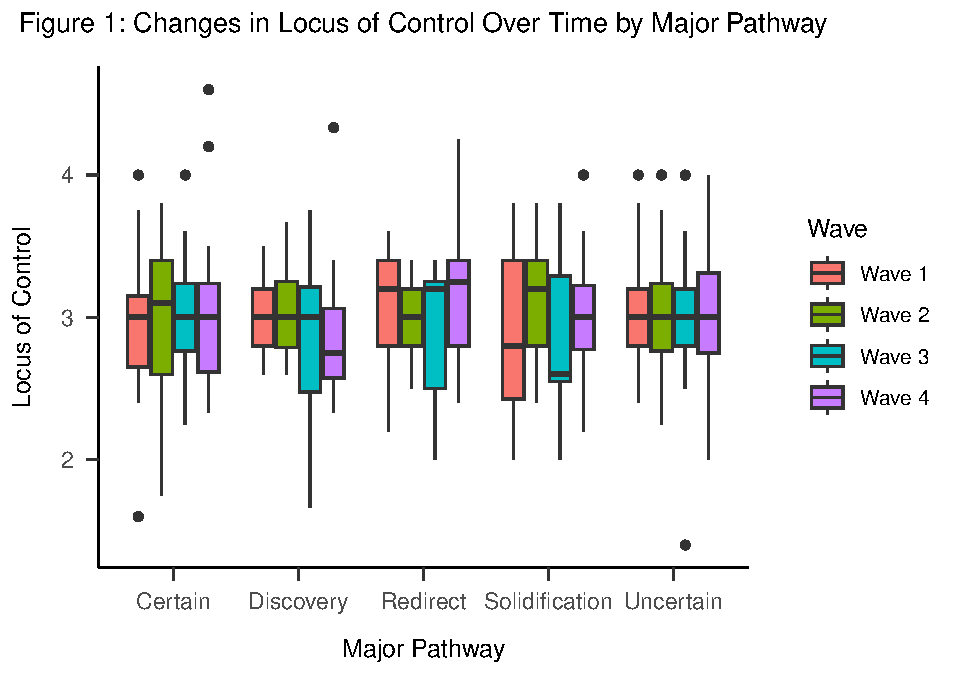
\includegraphics[keepaspectratio]{loc_pathways_report_2025-11-17_files/figure-latex/boxplot-1.pdf}}

\newpage

\section{References}\label{references}

\phantomsection\label{refs}
\begin{CSLReferences}{1}{0}
\bibitem[\citeproctext]{ref-R-papaja}
Aust, F., \& Barth, M. (2025). \emph{{papaja}: {Prepare} reproducible {APA} journal articles with {R Markdown}}. \url{https://doi.org/10.32614/CRAN.package.papaja}

\bibitem[\citeproctext]{ref-R-tinylabels}
Barth, M. (2025). \emph{{tinylabels}: Lightweight variable labels}. \url{https://doi.org/10.32614/CRAN.package.tinylabels}

\bibitem[\citeproctext]{ref-R-summarytools}
Comtois, D. (2025). \emph{Summarytools: Tools to quickly and neatly summarize data}. \url{https://doi.org/10.32614/CRAN.package.summarytools}

\bibitem[\citeproctext]{ref-cuxf4tuxe92016}
Côté, J. E., Mizokami, S., Roberts, S. E., \& Nakama, R. (2016). An examination of the cross-cultural validity of the Identity Capital Model: American and Japanese students compared. \emph{Journal of Adolescence}, \emph{46}(1), 76--85. \url{https://doi.org/10.1016/j.adolescence.2015.11.001}

\bibitem[\citeproctext]{ref-R-flextable}
Gohel, D., \& Skintzos, P. (2026). \emph{Flextable: Functions for tabular reporting}. \url{https://doi.org/10.32614/CRAN.package.flextable}

\bibitem[\citeproctext]{ref-gordon1998}
Gordon, V. N. (1998). Career Decidedness Types: A Literature Review. \emph{The Career Development Quarterly}, \emph{46}(4), 386--403. \url{https://doi.org/10.1002/j.2161-0045.1998.tb00715.x}

\bibitem[\citeproctext]{ref-magolda2023}
Magolda, M. B. B. (2023). \emph{Making their own way: Narratives for transforming higher education to promote self-development}. New York: Routledge. \url{https://doi.org/10.4324/9781003445883}

\bibitem[\citeproctext]{ref-nowicki2018}
Nowicki, S., Ellis, G., Iles-Caven, Y., Gregory, S., \& Golding, J. (2018). Events associated with stability and change in adult locus of control orientation over a six-year period. \emph{Personality and Individual Differences}, \emph{126}, 85--92. \url{https://doi.org/10.1016/j.paid.2018.01.017}

\bibitem[\citeproctext]{ref-R-base}
R Core Team. (2025). \emph{R: A language and environment for statistical computing}. Vienna, Austria: R Foundation for Statistical Computing. Retrieved from \url{https://www.R-project.org/}

\bibitem[\citeproctext]{ref-rose1971}
Rose, H. A., \& Elton, C. F. (1971). Attrition and the vocationally undecided student. \emph{Journal of Vocational Behavior}, \emph{1}(1), 99--103. \url{https://doi.org/10.1016/0001-8791(71)90011-X}

\bibitem[\citeproctext]{ref-R-DescTools}
Signorell, A. (2025). \emph{DescTools: Tools for descriptive statistics}. \url{https://doi.org/10.32614/CRAN.package.DescTools}

\bibitem[\citeproctext]{ref-spight2024}
Spight, D. B., Mooney, D., \& Orr, R. (2024). A historiographic review of the research on undecided students. \emph{NACADA Review}, \emph{4}(2), 78--91. \url{https://doi.org/10.12930/NACR-22-17}

\bibitem[\citeproctext]{ref-R-ggplot2}
Wickham, H. (2016). \emph{ggplot2: Elegant graphics for data analysis}. Springer-Verlag New York. Retrieved from \url{https://ggplot2.tidyverse.org}

\bibitem[\citeproctext]{ref-R-dplyr}
Wickham, H., François, R., Henry, L., Müller, K., \& Vaughan, D. (2023). \emph{Dplyr: A grammar of data manipulation}. \url{https://doi.org/10.32614/CRAN.package.dplyr}

\bibitem[\citeproctext]{ref-R-tidyr}
Wickham, H., Vaughan, D., \& Girlich, M. (2024). \emph{Tidyr: Tidy messy data}. \url{https://doi.org/10.32614/CRAN.package.tidyr}

\end{CSLReferences}


\end{document}
